% Chapter Template

\chapter{Data Pipeline} % Main chapter title

\label{Chapter3} % Change X to a consecutive number; for referencing this chapter elsewhere, use \ref{ChapterX}

This chapter describes the data pipeline, from downloading to analysis as shown in figure \ref{fig:pipelineFlowChart}. The data is hosted in bulk on the USPTO website \cite{USPTObulkdata}, after parsing the html of the website to extract the download urls and download the data it is parsed into two structured tables, one for information about each patent and another for each citation within each patent, i.e. a collection of edges along with some additional information to ease cross referencing strain later. After parsing the data is cleaned and tested to ensure a reasonable level of quality and to get a qualitative understanding of the accuracy and limitations of the data-set. From this point some analysis can be done on the data such as degree distribution or number of patents granted each year, for more in depth analysis feature engineering is done either in memory using R or through map-reduce and other database frameworks, for this reason the data is migrated from csv files to a database. Finally analysis is done on the feature engineered data, primarily this is done through using database frameworks to summarize or sample the data before exporting to R for the main analysis and graphical representation. 


\begin{figure}[ht]
\centering
  \centering
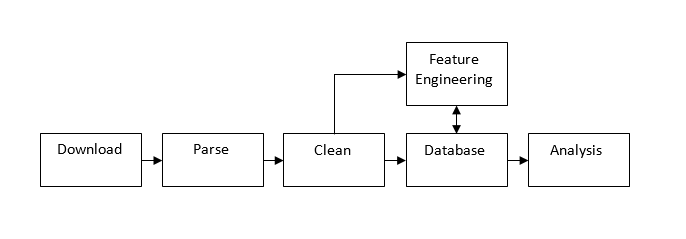
\includegraphics[width=0.7\linewidth]{Figures/FlowChart}
\caption[Flowchart: Data Pipeline]{\small Flowchart of the data pipeline}
\label{fig:pipelineFlowChart}
\end{figure}


%----------------------------------------------------------------------------------------
%	SECTION 1: Raw Data
%----------------------------------------------------------------------------------------

\section{Raw Data} \label{section: Raw Data}

The USPTO offers one of the largest openly available patent networks with images of their patents and trademark documents available since 1796; as text through optical character recognition since 1920 and more recently from 1976 structured full text data (excluding images and diagrams) is available. A subset of the full text data is the bibliographic data; all of the front page information such as date granted, the title of the patent and the citation information. 

This data-set from January 1st 1976 to December 31st 2015 is 110Gb in size in the form of a structured documents of varying formats: From 1976 to 2001 a proprietary text format is used, from 2002 onward the USPTO follows the Patent Grant International Common Element (ICE) document type definition (DTD). While ICE provides international consistency it revised frequently, initially using sgml (ICE 1.5 and 1.6) in 2005 switching to XML for versions 4.0 - 4.4 \cite{ICE}. One patent from each of the three major formats (text, sgml and xml) are included in appendix \ref{AppendixB}, \ref{AppendixC} and \ref{AppendixD} respectively. 

Up until 1996 each year contains one file containing all the patent information in that year in a single document. After this point there is a separate file for each week an associated file listing all the patent numbers present in that file and a summary file containing extra information such as notes about that week and the number of total patents granted of each type. The sgml and xml files have each patent as a single document appended into a single file. 

%-----------------------------------
%	SECTION 2: Parsing
%-----------------------------------
\section{Parsing} \label{section:parsing}

The above structure of the data presents a number of challenges to the parsing process. Most notably the changing formats and schema. The difficulty is parsing these in a consistent way, to minimise any systematic differences between the formats.

A single parsing function for all formats was developed; using the same functional structure to process each format  (Appendix \ref{AppendixA}). The core logical loop for parsing each line of data, shown in figure \ref{fig:FlowChartCoreLogic}, extracts the tag and contents of each line, where the tag is the expression identifying what the contents is, e.g. <date>20011004</date> indicates the contents between the brackets is a date. The function then maps the tag to an action and takes that action. This minimizes differences between formats as long as a semantically equivalent mapping can be found for each. 

The parsing function builds up two tables, one for the patent level data and one for the citations. Initializing each of these as empty vectors, adding patent information and citation information to those vectors and flushing them by appending them to a csv file at the end of each citation or patent section in the document \ref{fig:FlowChartParseStructure}. Some tags are not unique, such as date referring to the date a patent was granted the date a patent application was made or the date a citation patent was granted. To resolve this issue the function identifies the region of a patent document it is currently in and therefore how to interpret uniquely a non-unique tag. It also takes the opportunity to record the degree of each patent with a simple counter. 

The second philosophy of this method of parsing makes it easy to adjust the variables being recorded by adding the tags to the mapping vectors (and name), this flexibility handles changes in schema over time and parsing new variables. 

The variables parsed for each patent were: Patent number, degree, date granted, main and further classification codes. The variables extracted for each citation were: Parent patent number, citation patent number, citation patent granted date, country of the citation and 'cited by' which distinguishes between two classes of individual producing the citation. In this way the citations are in a tall format, in accordance with Hadley Wickham's principles of 'tidy data' \cite{wickham2014tidy}. 

\begin{figure}
\centering
\begin{subfigure}{.3\textwidth}
  \centering
  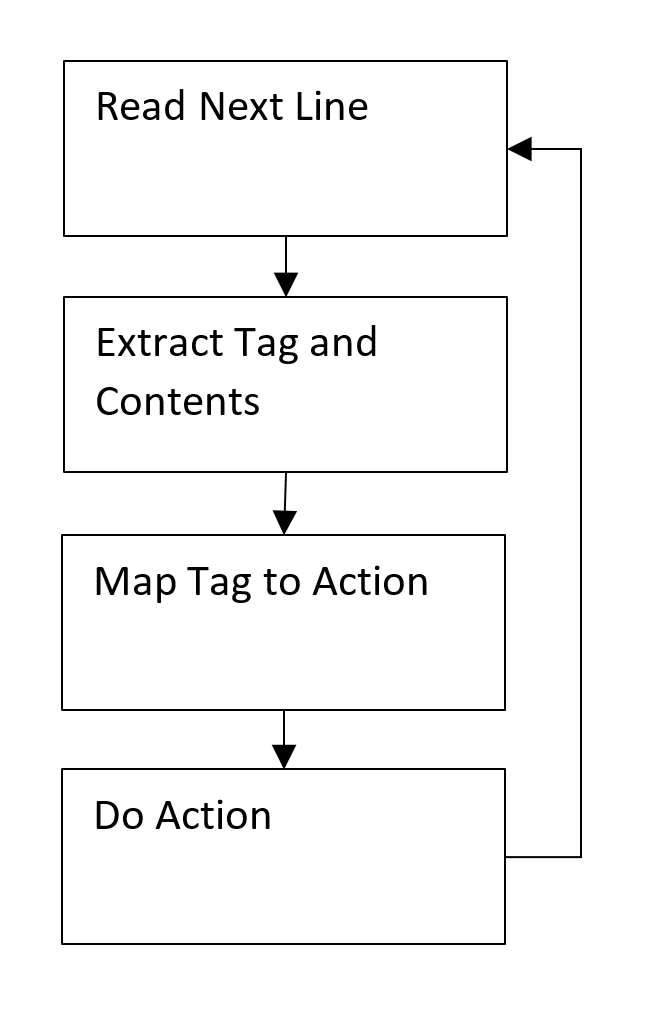
\includegraphics[width=0.7\linewidth]{Figures/FlowChartCoreLogic}
  \caption{}
\label{fig:FlowChartCoreLogic}
\end{subfigure}%
\begin{subfigure}{.7\textwidth}
  \centering
  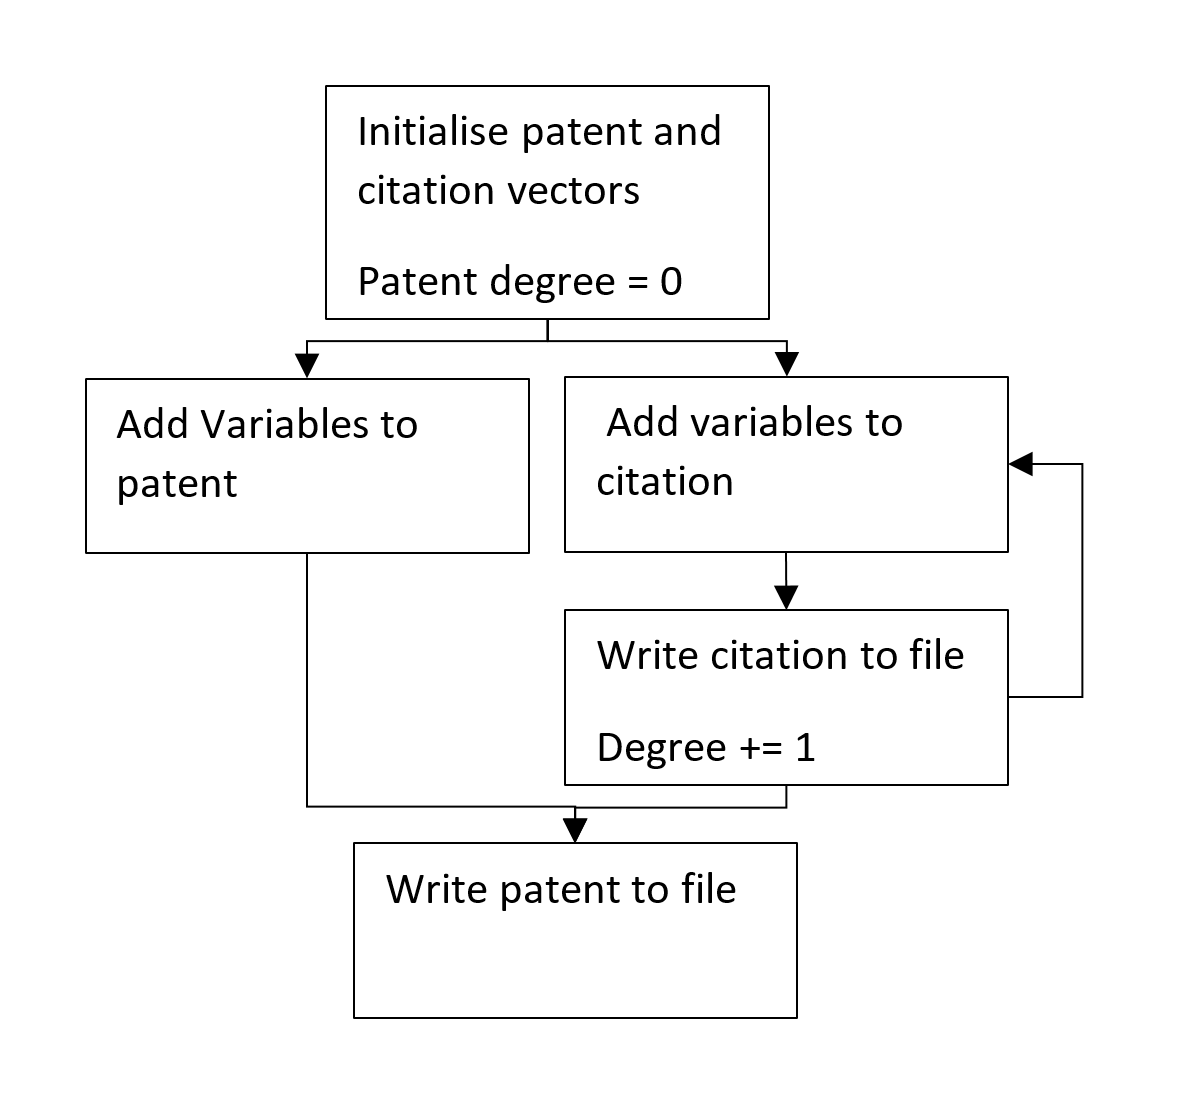
\includegraphics[width=0.7\linewidth]{Figures/FlowChartParseStructure}
  \caption{}
\label{fig:FlowChartParseStructure}
\end{subfigure}
\caption[Flowchart: Parsing Function]{\footnotesize Flowchart showing the structure of the document parsing function. (A) describes the logical loop while (B) describes the structure in which a whole patent is parsed into a patent Vector and a citation table}
\label{fig:Structure of Parsing Algorithm}
\end{figure}

%-----------------------------------
%	SUBSECTION 1: Cleaning
%-----------------------------------

\subsection{Cleaning} \label{section:Cleaning}

After parsing the data it is cleaned to remove some sources of systematic errors. Dealing with big data, considerations must be made when cleaning the data with respect to the impact compared to the difficulty performing that cleaning. The data is tested against some reference points to assess its consistency, both internally between different formats and schema and externally against other sources. 

The categorical factors such as 'citedBy' and 'Country' are cleaned by generating a list of possible values that factor can take and excluding values outside those levels. The dates are in a numeric format "YYYYMMDD" (Where Y,M,D refers to digits representing Year, Month and Day respectively). This is parsed into a date object represented by the number of days since the 1st of January 1970. This allows the dates to be more directly compared as they can be subtracted to get time differences. This process also isolates any values which do not conform to the expected format and returns NA. Using 2001 as an example only 1 date failed to parse this way. Dates on the patents must also in the range of 1976 and 2015. Citation dates can be lower as patents may cite other patents which are not in our data-set. 

Technology codes and patent numbers follow specific schema, US patent numbers are numeric codes which may have a preceding letter (D|RE|PP| H|T) indicating their class, e.g. 'D' represents design patents. While it can be ensured that all US patents use this schema there are foreign patents with many different schema, it is impractical to clean for all these foreign patent schema. In practice not cleaning these foreign patent numbers is unlikely to have an impact on the analysis as the primary purpose for cleaning these patent numbers is to improve matches between citations and patents, which is only necessary for internal citations.  

The patent numbers under citations had several encoding inconsistencies with those under the Patent: punctuation, white-space, additional filler '0' characters and additional digits at the end of the number when parsed from the text format were all cleaned. In 2001 94.5\% of the US citations after 1976 were matched with patents parsed. 

There are a variety of sources of NA values in the dataset. In the parsing phase missing data in the raw dataset is returned as NA and when reading the outputted csv each value must be the expected type (e.g. Order must be an integer). The cleaning phase also produces NA values when a factor value doesn't fit into allowed levels. For example in 2001 4 citations were completely NA, 155 numeric dates are NA and 897 dates when parsed into date format are NA. That year there are a total of 2,609,494 citations so NA values are negligible in quantity. 

The parsed and cleaned data can be compared to those published by the USPTO \cite{USPTOSummary}, as well as the number of patents in the '.lst' files which mirror the raw files documenting the patent numbers present. If accurate, differences between these files and parsed patents represent the patents that the parsing function has failed to process. '.lst' files are only available from 1997 onward (figure \ref{fig:patentCountsTest}). There are two large differences between patent counts at either end of the data-set; in 1976 and 2016. The difference in 2016 is due to two weeks of data having access denied during the download stage but all the weeks are present in 1976 so the difference here is unknown. Due to the relative size of these errors these years have been omitted from patent count based analysis. Before 2008 the number of patents parsed was equivalent to the USPTO summary statistics, since then however the parsed data has significantly more patents than present in the summary statistics. Manually looking up some of these additional patents reveals them to be complete non-duplicated patents so it is not clear why they may be missing. There have always been a small number of patents in the list files not parsed, however until approximately 2010 these numbers were fewer than 100 but have grown to around 1\% of the data, this aligns with the summary statistics divergence suggesting they also experienced these problems to a more severe degree. The difference here doesn't line up with the introduction of XML (2005) but may be due to some of the ICE schema changes or errors in the structure of the document (trying to use an XML parsing library on these years yielded a lot of missing data due to failure to structural errors in the XML). 

\begin{figure}
\centering
\begin{subfigure}{\textwidth}
  \centering
  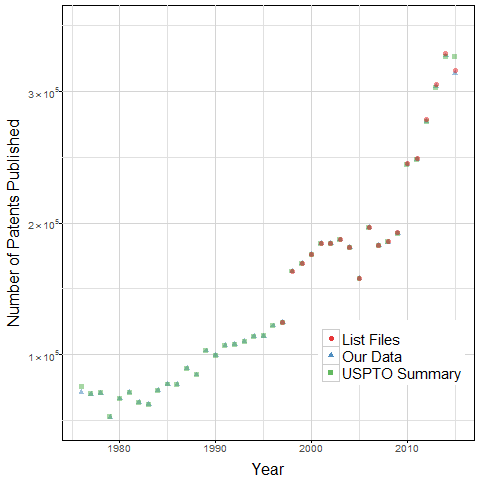
\includegraphics[width=0.9\linewidth]{Figures/patentsCompared}
 \caption{Number of Patents parsed each year from each source}
\label{fig:patentsCompared}
\end{subfigure}%
\\
\begin{subfigure}{\textwidth}
  \centering
  
\includegraphics[width=0.7\linewidth]{Figures/patentsDiff}
  \caption{\footnotesize Difference between number of Patents parsed from different sources and parsed data}
\label{fig:patentsDiff}
\end{subfigure}
\caption[Difference between number of patents parsed from different sources]{\footnotesize The number of Patents granted each year according to 3 sources: Parsed data; a USPTO report and the .lst files.}
\label{fig:patentCountsTest}
\end{figure}

The second reference point for parsing the data is internal consistency. In 2001 both text and sgml data files are present. This gives the unique opportunity to parse both and compare the results. We found that 95 / 184078 patents are present in the text parsing but absent in the sgml, but none are present in the sgml and absent in the text format. Manually referencing the patent numbers with the USPTO database reveals they are valid patents missed absent from the sgml document rather than missed from the parsing method. When these patents are taken into account all citations are present in both formats. Overall these differences confirm that although there are some differences in the raw data, the parsing function is treating differing data formats equally.


%----------------------------------------------------------------------------------------
%	SECTION 3: Database processing
%----------------------------------------------------------------------------------------

\section{Database processing}

Once the data has been parsed and cleaned some analysis can be done on it, but most analysis requires feature engineering. Because the data does not fit in memory this can be done in batch but often the data must be reordered or regrouped, for this reason a database was used. Mongodb was chosen for this as it is designed around big data with its map-reduce and aggregation frameworks making these feature engineering operations to be done in parallel, having javascript and JSON as primary interfaces allowed for ease of use. 

\begin{figure}
\centering
\begin{subfigure}{.5\textwidth}
  \centering
  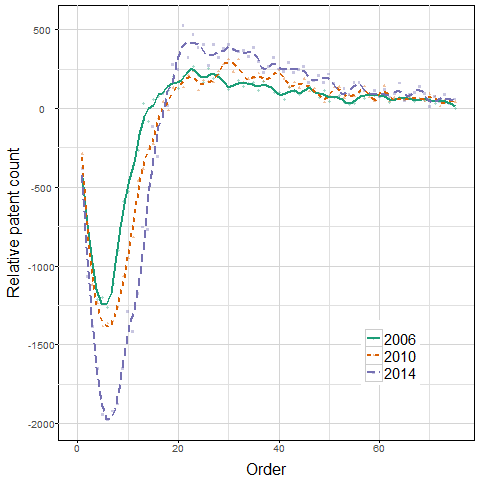
\includegraphics[width=.9\linewidth]{Figures/parsingErrorsPerOrder}
 \caption[]{}
\label{fig:parsingErrorsPerOrder}
\end{subfigure}%
\begin{subfigure}{.5\textwidth}
  \centering
  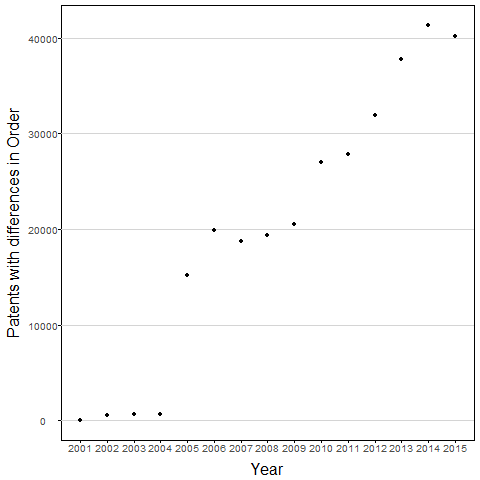
\includegraphics[width=0.9\linewidth]{Figures/parsingErrorsPerYear}
  \caption[]{}
\label{fig:parsingErrorsPerYear}
\end{subfigure}
\caption[Differences in different parsing methods]{Number of patents with different order based on parsing method. (A) against order for the years 2006, 2010 and 2014 and (B) for each year.}
\label{fig:parsingErrors}
\end{figure}

Using a map-reduce the order for each patent was calculated as the number of citations matching each patent. There are some differences between these orders and the ones produced with the parsing function (figure \ref{fig:parsingErrors}).  We can see that these differences are only non-negligible after 2005, when the XML format is introduced. Manual inspection shows that the map-reduced orders are the ones which are incorrect but it is not obvious what the cause of the error is. The map-reduce over represents small orders and under-represents large orders, with the same total number of citations parsed. This suggests that the map-reduce may be interpreting a single patent as multiple different patents. This error only becomes significant in the most recent years but represents 1\% of the data in 2015, so caution is advised for these years. 

In summary the parsing and cleaning of the data have focused heavily on maximizing the consistency of the data parsed from the design of the parsing function to the cleaning steps. We have analysed these results and find that it out-performs USPTO summary statistics and non-negligible errors appear to be limited to 1976 and the last few years of the data-set. It is important to know where these errors are and be cautious when analysing them but we can't dismiss these sections of the data-set.